% Part: sets-functions-relations
% Chapter: infinite
% Section: hilberts-hotel
%
\documentclass[../../../include/open-logic-section]{subfiles}

\begin{document}

\olfileid{sfr}{infinite}{hilbert}
\olsection{Hilbert旅馆}

自然数集显然是无穷的。所以，如果我们不想\emph{直接诉诸}自然数，那么第一步就必须用不涉及自然数本身的术语来刻画无穷集合。这里有一个很好的方法，由 Hilbert（希尔伯特） 在 1924 年的一次讲座中提出。他让我们想象

\begin{quote}
[\ldots] 一个拥有有限个房间的旅馆。每间房都应当恰好住着一位客人。如果现在客人以某种方式调换房间，[但]使得每个房间仍然至多只有一个人，那么不会有任何房间空出来，旅馆主人也就无法通过这种方式为新到来的客人腾出新的位置[\ldots \textparagraph \ldots]

现在我们规定，这个旅馆拥有无穷多个编号为 $1$， $2$， $3$， $4$， $5$， \dots 的房间，其中每个房间都恰好住着一位客人。一旦有新客人到来，旅馆主人只需要把每位老客人移到房号大~$1$ 的房间里，那么房间~$1$ 就会空出来给新到来的客人。
	\begin{center}
		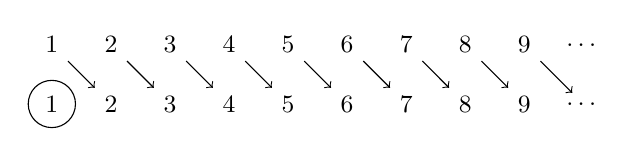
\begin{tikzpicture}[scale = .75]
		\foreach \x in {1, 2, 3, 4, 5, 6, 7, 8, 9}
		{
			\node (\x a) at (\x, 1) {\small{\x}};
			\node (\x b) at (\x, 2) {\small{\x}};
		}
		\node (dotsa) at (10, 1) {\small{\ldots}};
		\node (dotsb) at (10, 2) {\small{\ldots}};
		\draw[->] (1b)--(2a);
		\draw[->] (2b)--(3a);
		\draw[->] (3b)--(4a);
		\draw[->] (4b)--(5a);
		\draw[->] (5b)--(6a);
		\draw[->] (6b)--(7a);
		\draw[->] (7b)--(8a);
		\draw[->] (8b)--(9a);
		\draw[->] (9b)--(dotsa);
		\draw (1,1) circle (.4);
		\end{tikzpicture}
	\end{center}
	（发表于 \citealt[730]{EwaldSieg2013}；由我们翻译）
\end{quote}

关键点在于，Hilbert旅馆拥有无穷多个房间；我们可以把他的解释用来定义“拥有无穷多”意味着什么。事实上，这正是 Dedekind 的进路（当然，这里的呈现有着严重的时代错位；Dedekind 的定义来自 \citeyear{Dedekind1888}）：

\begin{defn}\ollabel{defn:DedekindInfinite}
集合 $A$ 是 \emph{Dedekind 无穷的}，当且仅当存在一个从~$A$ 到其真子集的单射。
也就是说，存在某个 $o \in A$ 以及一个单射 $f \colon A \to A$，使得 $o \notin \ran{f}$。
\end{defn}

\end{document}